
\documentclass{article}
\usepackage{graphicx} % Required for inserting images
\usepackage{amsmath,amssymb,enumerate,graphicx,pgf,tikz,fancyhdr}
\usetikzlibrary{backgrounds}
\usepackage{geometry}
\usepackage{tabvar}
\usepackage{fontspec}
\usepackage{minted}



\geometry{hmargin=2.2cm,vmargin=1.5cm}

\title{TP 1: Parcours d'Arbre Binaire}
\author{HACINI Malik}
\date{13 Septembre 2023}
\renewcommand{\contentsname}{Table des Matières}
\begin{document}

\maketitle
\tableofcontents{}

\section{Introduction}

Le but de ce TP est de représenter un arbre binaire en python via une classe,
puis de le parcourir en profondeur de 3 façons différentes.




\section{Classe "Noeud"}
Voici l'implémentation de la classe Noeud.
Chaque noeud a pour attribut l'information qu'il porte (un entier) 
et ses fils gauches et droits, d'autres noeuds.
On ajoute aussi les Méthode d'instance de classe ajouter-d et ajouter-g, qui
permettent de créer un noeud, fils gauche ou droit d'un autre.

\renewcommand{\theFancyVerbLine}{
  \sffamily\textcolor[rgb]{0.5,0.5,0.5}{\scriptsize\arabic{FancyVerbLine}}}

\begin{minted}[mathescape,
               linenos,
               numbersep=5pt,
               gobble=2,
               frame=lines,
               framesep=2mm]{python}
    from __future__ import annotations

  class Noeud:
    def __init__(self,info=int,f_g=None,f_d=None):
        self.info=info
        self.f_g=f_g
        self.f_d=f_
        
    #Ajoute un noeud a l'arbre, en tant que fils de son père (self)

    def ajouter_d(self,info):
        self.f_d = Noeud(info)
        return self.f_d
    
    def ajouter_g(self,info):
        self.f_g = Noeud(info)
        return self.f_g

\end{minted}

\section{Construction de l'Arbre}

\subsection{Schéma}
\begin{center}
\resizebox {\textwidth} {!} {

 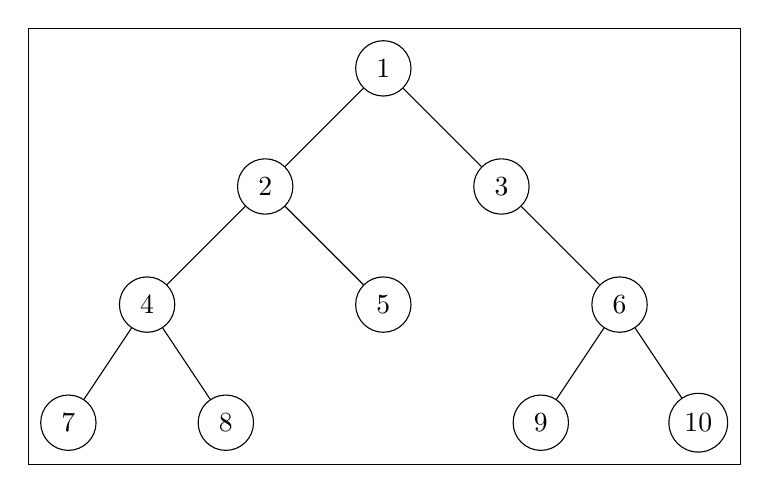
\begin{tikzpicture}[framed,
    every node/.style = {
    minimum width = 2em, draw, circle},
    level/.style = {sibling distance = 30mm/#1}
    ]
    \node {1}
    child {node {2} 
          child {node {4}
          child{node{7}}
          child{edge from parent[draw = none]}
          child{node{8}}}
          child {edge from parent[draw = none]}
          child {node {5}}
          }
    child {node {3}
           child {edge from parent[draw = none]
           }
           child {edge from parent[draw = none]}
           child {node {6}
                   child {node {9}}
                   child {edge from parent[draw = none]}
                   child {node {10}}}
            };
 \end{tikzpicture}}
\end{center}
Nous allons travailler avec cet arbre binaire (non strict). Il sera efficace pour les tests, car il 
comporte tout les types de noeuds possibles.
\subsection{Implémentation.}
On construit l'arbre de haut en bas, à l'aide de la classe Noeud.
\renewcommand{\theFancyVerbLine}{
  \sffamily\textcolor[rgb]{0.5,0.5,0.5}{\scriptsize\arabic{FancyVerbLine}}}

\begin{minted}[mathescape,
               linenos,
               numbersep=5pt,
               gobble=2,
               frame=lines,
               framesep=2mm]{python}
    n1=Noeud(1)
    n2=n1.ajouter_g(2)
    n3=n1.ajouter_d(3)
    n4=n2.ajouter_g(4)
    n5=n2.ajouter_d(5)
    n6=n3.ajouter_d(6)
    n7=n4.ajouter_g(7)
    n8=n4.ajouter_d(8)
    n9=n6.ajouter_g(9)
    n10=n6.ajouter_d(10)
\end{minted}

\newpage
\section{Parcours de l'Arbre}
 Il y a 3 types de parcours en profondeur : préfixe, postfixe et infixe.
 Chacun de ces parcours correspond à un ordre différent.
 Pour chacun d'entre eux, on l'implémente de deux façons différentes :
 \newline
 -Une en tant que méthode d'instance de la classe Noeud
 \newline
 -Une en tant que fonction extérieure à la classe
\subsection{Préfixe}
Le parcours préfixe consiste à parcourir l'arbre suivant l'ordre : r --> fils g. --> fils d.
 Pour notre arbre, il correspond au parcours dans 
 l’ordre 1 - 2 - 4 - 7 - 8 - 5 - 3 - 6 - 9 - 10 , 
 c’est à dire suivant le premier passage à \textbf{gauche} d’un nœud.
\renewcommand{\theFancyVerbLine}{
  \sffamily\textcolor[rgb]{0.5,0.5,0.5}{\scriptsize\arabic{FancyVerbLine}}}

\begin{minted}[mathescape,
               linenos,
               numbersep=5pt,
               gobble=2,
               frame=lines,
               framesep=2mm]{python}
    #Méthode d'instance de classe

    def prefixe(self)->list:
        info=[self.info]
        if self.f_g!= None:
            info= info + self.f_g.prefixe()
        if self.f_d!= None:
            info= info + self.f_d.prefixe() 
        return info

    #Fonction extérieure

    def parcours_prefixe(n=Noeud)->list:
        if n is None:
            return []
        
        return [n.info] + parcours_prefixe(n.f_g) + parcours_prefixe(n.f_d)


\end{minted}
\subsection{Postfixe}
Le parcours postfixe consiste à parcourir l'arbre suivant l'ordre : fils g. --> fils d. --> r
 Pour notre arbre, il correspond au parcours dans 
 l’ordre 7 - 8 - 4 - 5 - 2 - 9 - 10 - 6 - 3 - 1 ,
 c'est à dire suivant le premier passage à \textbf{droite} d'un noeud.

\renewcommand{\theFancyVerbLine}{
  \sffamily\textcolor[rgb]{0.5,0.5,0.5}{\scriptsize\arabic{FancyVerbLine}}}

\begin{minted}[mathescape,
               linenos,
               numbersep=5pt,
               gobble=2,
               frame=lines,
               framesep=2mm]{python}
    #Méthode d'instance de classe
    def postfixe(self)->list:
        info=[]
        if self.f_g!=None:
            info= info + self.f_g.postfixe()  
            
        if self.f_d!=None:
            info= info + self.f_d.postfixe()
        info = info + [self.info]
        return info

    #Fonction extérieure

    def parcours_postfixe(n=Noeud)->list:
        if n is None:
            return []
        
        return parcours_postfixe(n.f_g) + parcours_postfixe(n.f_d) + [n.info]
\end{minted}
\newpage
\subsection{Infixe}
Le parcours infixe consiste à parcourir l'arbre suivant l'ordre : fils g. --> r --> fils d.
 Pour notre arbre, il correspond au parcours dans 
 l’ordre 7 - 4 - 8 - 2 - 5 - 1 - 3 - 9 - 6 - 10,
 c'est à dire suivant le premier passage \textbf{sous} un noeud.
\renewcommand{\theFancyVerbLine}{
  \sffamily\textcolor[rgb]{0.5,0.5,0.5}{\scriptsize\arabic{FancyVerbLine}}}

\begin{minted}[mathescape,
               linenos,
               numbersep=5pt,
               gobble=2,
               frame=lines,
               framesep=2mm]{python}
    #Méthode d'instance de classe

    def infixe(self)->list:
    info=[]
    if self.f_g!=None:
        info= info + self.f_g.infixe() 
         
    info = info + [self.info]
    
    if self.f_d!=None:
        info= info + self.f_d.infixe()
    return info
    
    #Fonction extérieure
    def parcours_infixe(n=Noeud)->list:
    if n is None:
        return []
    return parcours_infixe(n.f_g) + [n.info] + parcours_infixe(n.f_d)

\end{minted}
%\newpage  

\section{Tests}
On écrit 3 tests, un dédié à chaque parcours.
Chaque test est séparé en 2 parties: l'une pour la méthode et l'autre pour la fonction associé au parcours.
Pour s'assurer du bon fonctionnement du programme, on teste 4 noeuds de types différents :
\newline
- Le noeud 1, racine de l'arbre
\newline
- Le noeud interne 4
\newline
- Les feuilles 5 et 9, à deux hauteurs différentes.
\subsection{Préfixe}


\renewcommand{\theFancyVerbLine}{
  \sffamily\textcolor[rgb]{0.5,0.5,0.5}{\scriptsize\arabic{FancyVerbLine}}}

\begin{minted}[mathescape,
               linenos,
               numbersep=5pt,
               gobble=2,
               frame=lines,
               framesep=2mm]{python}

    #Méthode d'instance de classe

    def test_prefixe_classe():
        
        assert n1.prefixe()==[1, 2, 4, 7, 8, 5, 3, 6, 9, 10]
        assert n4.prefixe()==[4, 7, 8]
        assert n5.prefixe()==[5]
        assert n9.prefixe()==[9]

    #Fonction extérieure

    def test_prefixe_fonction():
    
        assert parcours_prefixe(n1)==[1, 2, 4, 7, 8, 5, 3, 6, 9, 10]
        assert parcours_prefixe(n4)==[4, 7, 8]
        assert parcours_prefixe(n5)==[5]
        assert parcours_prefixe(n9)==[9]
\end{minted}
\newpage
\subsection{Postfixe}

\renewcommand{\theFancyVerbLine}{
  \sffamily\textcolor[rgb]{0.5,0.5,0.5}{\scriptsize\arabic{FancyVerbLine}}}

\begin{minted}[mathescape,
               linenos,
               numbersep=5pt,
               gobble=2,
               frame=lines,
               framesep=2mm]{python}
    #Méthode d'instance de classe

    def test_postfixe():
        assert n1.postfixe()==[7, 8, 4, 5, 2, 9, 10, 6, 3, 1]
        assert n4.postfixe()==[7, 8, 4]
        assert n5.postfixe()==[5]
        assert n9.postfixe()==[9]

    #Fonction extérieure

    def test_postfixe_fonction():
    
        assert parcours_postfixe(n1)==[7, 8, 4, 5, 2, 9, 10, 6, 3, 1]
        assert parcours_postfixe(n4)==[7, 8, 4]
        assert parcours_postfixe(n5)==[5]
        assert parcours_postfixe(n9)==[9]
    


\end{minted}

\subsection{Infixe}

\renewcommand{\theFancyVerbLine}{
  \sffamily\textcolor[rgb]{0.5,0.5,0.5}{\scriptsize\arabic{FancyVerbLine}}}

\begin{minted}[mathescape,
               linenos,
               numbersep=5pt,
               gobble=2,
               frame=lines,
               framesep=2mm]{python}
    #Méthode d'instance de classe

    def test_infixe():
        assert n1.infixe()==[7, 4, 8, 2, 5, 1, 3, 9, 6, 10]
        assert n4.infixe()==[7, 4, 8]
        assert n5.infixe()==[5]
        assert n9.infixe()==[9]

    #Fonction extérieure

    def test_infixe_fonction():
    
        assert parcours_infixe(n1)==[7, 4, 8, 2, 5, 1, 3, 9, 6, 10]
        assert parcours_infixe(n4)==[7, 4, 8]
        assert parcours_infixe(n5)==[5]
        assert parcours_infixe(n9)==[9]
\end{minted}
\subsection{Résultats}
Pytest valide tout les tests.
\end{document} 
